\documentclass[sigconf]{acmart}

\usepackage{booktabs} % For formal tables
\usepackage{todonotes}
\usepackage[inline]{enumitem}

%%%%%% Standard Packages %%%%%%
\usepackage{graphicx}
\usepackage{amssymb}
%\usepackage[noend]{algorithmic}
\usepackage{algorithm}
\usepackage{stackrel}
\usepackage{algpseudocode}
\usepackage{textcomp}
\PassOptionsToPackage{table}{xcolor}
\usepackage[table]{xcolor}
\usepackage{listings}
\usepackage{subcaption}
% \usepackage{caption}
\usepackage{amsmath}
\usepackage{mathtools,xparse}
\usepackage{dsfont}
\usepackage{stmaryrd}
% \usepackage[inline]{enumitem}

%\usepackage{cite}
\usepackage{paralist}
\usepackage{hyperref}
\usepackage{cleveref}
\usepackage{lipsum}
\usepackage[normalem]{ulem}
\usepackage{array}
\usepackage{multicol}
\usepackage{enumitem}
\usepackage{etoolbox}
\usepackage{varwidth}
\usepackage{xspace}

\usepackage{multirow}
\usepackage{float}

%%%%%% Package Configuration %%%%%%
%%% Listings
\lstset{language=sql,morekeywords={LENS,SCHEMA_MATCHING,string},basicstyle=\small\upshape\ttfamily,keywordstyle=\color{blue}}
%%% verbatim
\makeatletter
\preto{\@verbatim}{\topsep=5pt \parsep=0pt }
\makeatother
%%% Algorithmic
\renewcommand{\algorithmicrequire}{\textbf{In:}}
\renewcommand{\algorithmicensure}{\textbf{Out:}}
%% Multicol
\setlength\multicolsep{\topsep}

%%%%%% Standard Theorem Environments %%%%%%
%\newtheorem{example}{Example}
\newtheorem{scenario}{Scenario}
%\newtheorem{definition}{Definition}
\newtheorem{property}{Property}
\newtheorem{transformation}{Transformation}

%%%%%%% Table styling %%%%%%
\newcolumntype{L}[1]{>{\raggedright\let\newline\\\arraybackslash\hspace{0pt}}m{#1}}
\newcolumntype{C}[1]{>{\centering\let\newline\\\arraybackslash\hspace{0pt}}m{#1}}
\newcolumntype{R}[1]{>{\raggedleft\let\newline\\\arraybackslash\hspace{0pt}}m{#1}}


%%%%%% Common Math-Mode Aliases %%%%%%
\newcommand{\comprehension}[2]{\left\{\left.\;{#1}\;\right|\;{#2}\;\right\}}
%\newcommand{\bagcomprehension}[2]{\llbrace\left.\;{#1}\;\right|\;{#2}\;\rrbrace}
\newcommand{\bagcomprehension}[2]{\left\{\!\left|\left.\;{#1}\;\right|\;{#2}\;\right|\!\right\}}
\newcommand{\setsize}[1]{\left|#1\right|}
\newcommand{\tuple}[1]{\left<\;{#1}\;\right>}
\newcommand{\ordefn}{\;|\;}
\newcommand{\sch}[1]{\texttt{schema}({#1})}
\newcommand{\projection}{\pi}
\newcommand{\selection}{\sigma}
\newcommand{\logicalAnd}{\wedge}
\newcommand{\logicalOr}{\vee}
\newcommand{\Union}{\bigcup}
\newcommand*{\Unionl}{\Union\limits}
\newcommand{\Intersection}{\bigcap}
\newcommand{\E}{\mathrm{E}}
\newcommand{\expect}{\mathbb{E}}
\newcommand{\defineeq}{\overset{def}{=}}

\newcommand{\entropy}{\mathcal{H}}

\newcommand{\distinct}[1]{\lfloor{#1}\rfloor}

\DeclareMathOperator*{\argmin}{arg\,min}
\newcommand*{\argminl}{\argmin\limits}

\DeclareMathOperator*{\argmax}{arg\,max}
\newcommand*{\argmaxl}{\argmax\limits}

\DeclareMathOperator*{\mysum}{\sum}
\newcommand*{\mysuml}{\mysum\limits}

\DeclareMathOperator*{\myPi}{\Pi}
\newcommand*{\myPil}{\myPi\limits}

\DeclareMathOperator*{\mymin}{\min}
\newcommand*{\myminl}{\mymin\limits}

\DeclareMathOperator*{\mymax}{\max}
\newcommand*{\mymaxl}{\mymax\limits}

\DeclareMathOperator*{\myunion}{\bigcup}
\newcommand*{\myunionl}{\myunion\limits}

\renewcommand{\vec}[1]{\mathbf{#1}}

\DeclarePairedDelimiter{\norm}{\lVert}{\rVert}

%%%%%% TODOs %%%%%%
\newcommand{\placeholder}[1]{\textcolor{red}{[[ #1 ]]}}

%%%%%% Other Aliases %%%%%%
\newcommand{\ccomment}[1]{{\small\texttt{/*} #1 \texttt{*/}}}
\newcommand{\tinysection}[1]{\smallskip \noindent \textbf{#1.}~}
%\newcommand{\keyword}[1]{\textcolor{blue}{\texttt{#1}}}



\newcommand{\namesymbol}{\eta}

% Copyright
\setcopyright{none}
%\setcopyright{acmcopyright}
%\setcopyright{acmlicensed}
% \setcopyright{rightsretained}
%\setcopyright{usgov}
%\setcopyright{usgovmixed}
%\setcopyright{cagov}
%\setcopyright{cagovmixed}


% DOI
\acmDOI{10.475/123_4}

% ISBN
\acmISBN{123-4567-24-567/08/06}

%Conference
\acmConference[HILDA]{Human-in-the-Loop Data Analytics}{June 2018}{Houston Texas}
\acmYear{2018}
\copyrightyear{2018}


\acmArticle{4}
\acmPrice{15.00}



\newcommand{\systemname}{\textbf{LOKI}\xspace}

% These commands are optional
%\acmBooktitle{Transactions of the ACM Woodstock conference}
% \editor{Jennifer B. Sartor}
% \editor{Theo D'Hondt}
% \editor{Wolfgang De Meuter}

\begin{document}
\title{Building a Knowledgebase for Incremental Schema Recovery}
% \titlenote{Produces the permission block, and copyright information}
% \subtitle{Extended Abstract}
% \subtitlenote{The full version of the author's guide is available as \texttt{acmart.pdf} document}


\author{Poonam Kumari}
\affiliation{%
  \institution{University at Buffalo, SUNY}
}
\email{poonamku@buffalo.edu}

\author{Gourab Mitra}
% \orcid{1234-5678-9012}
\affiliation{%
  \institution{University at Buffalo, SUNY}
}
\email{gourabmi@buffalo.edu}

\author{Oliver Kennedy}
\affiliation{%
  \institution{University at Buffalo, SUNY}
}
\email{okennedy@buffalo.edu}


% The default list of authors is too long for headers.
\renewcommand{\shortauthors}{Kumari et al.}


\begin{abstract}
% -*- root: ../paper.tex -*-
There are few things sadder than an unlabeled (or poorly labeled) dataset.
Without names, data access becomes inordinately more difficult or even impossible.
In this paper we describe the first steps towards building a new tool that makes it easier for users to properly label data, and to help preserve those labels for future use.
Specifically, we outline the design of \systemname, a knowledge-base for storing column-naming heuristics, as well as an interactive tool: the \systemname editor for populating the knowledge-base.  
The \systemname editor primes the knowledge base by learning from example data (e.g., from open data portals), and assists domain experts in reviewing and refining the resulting heuristic naming schemes.
We identify specific issues arising from training and show how the \systemname editor streamlines the process of manually repairing these issues.

\end{abstract}

%
% The code below should be generated by the tool at
% http://dl.acm.org/ccs.cfm
% Please copy and paste the code instead of the example below.
%

\keywords{Schema Design, Knowledge Base, Data Loading, ETL}

\maketitle

\section{Introduction}
\label{sec:introduction}
% -*- root: ../paper.tex -*-

It's a story as old as time: A student gathers data, makes a graph with the data, writes a paper about the data.
Then the student graduates and the data languishes, without so much as a wiki page or README file documenting it.
The next student to use the data needs to spend hours, days, or even weeks reverse-engineering it.
Then they also graduate and the whole process can start over again.

As a way to break this tragic cycle of data abandonment, we propose \emph{Label Once, and Keep It} (\systemname), a data-ingest middleware for incremental, re-usable schema recovery.
\systemname allows users to assemble schemas on-demand, both (re-)discovering and incrementally refining schema definitions in response to changing data needs.  
To accomplish this, \systemname is built around a knowledge-base of both approximate, as well as exact schema labelings.
First, approximate labelings derived from existing open-data sets, user-feedback, and expert-provided heuristics, jump-start the labeling process.
When a user first points \systemname at a new tabular data set, \systemname provides users with a preliminary, default schema.
As users confirm and/or override parts of the proposed schema, \systemname preserves the labels for the dataset's next user.

The effectiveness of \systemname depends primarily on the quality of its knowledge-base.  
Hence, a properly populated konwledge-base is of paramount importance.
In this paper, we introduce the \systemname editor, a tool being developed as part of \systemname for exactly this purpose.
The \systemname editor allows knowledge to be incorporated into the knowledge-base in two ways: (1) By learning from example data (e.g., drawn from open data portals), and (2) By manual adjustment from domain experts.
In particular, we focus on the challenge of manual refinement of knowledge learned from example data.
The editor is designed to help experts to quickly identify and resolve errors and ambiguity in the \systemname knowledge-base.

Concretely, the contributions of this paper include:
\begin{enumerate*}
  \item We introduce \systemname in Section~\ref{sec:system} and detail the structure of its knowledge-base in Section~\ref{sec:knowledgebase}
  \item We illustrate how the \systemname editor pre-populates the knowledge-base by learning from example data in Section~\ref{sec:trainbyexample}.
  \item We identify specific errors that arise in the training process and show how the \systemname editor facilitates efficient detection and manual repair of the error.
\end{enumerate*}

% One more thought regarding a pitch for the work.  We could wrap the idea in the context of a larger system for importing / querying initially unlabeled data.  Specifically, when someone first loads an unlabeled (or only partially labeled) CSV file into a database/spark, they have two problems:

% 1) They need to label a subset of the columns that pertain to the specific analysis they want to do now.
% 2) They don't need to label *all* of the columns (might be 10s, 100s, or 1000s of columns that they don't care about).  

% However, at some point in the future, more labeling might be helpful.  For example:
% 1) They pose a query and randomly discover that they are missing a column that *could* potentially exist in the source data.
% 2) Someone else wants to use the same data set, but with a different selection of columns.
% 3) The knowledge-base is updated and more automatic labelings become available.

% I'm going to suggest that we present our contribution in the context of a system that:
% 1) Auto-suggests names for columns based on existing heuristics
% 2) Saves labeling efforts, making it possible to incrementally label a data-set and re-use effort across analyses
% 3) Allows you to ask whether a particular column name *could* exist in a given data set, and identify the data column that most-likely represents it.

% Specifically, in this paper, we're conducting a case study evaluating one particular approach to task (1).  

\section{System Design}
\label{sec:system}
% -*- root: ../paper.tex -*-
System Overview


Things we need to address:
\begin{itemize}
  \item How is this a ``middleware''  Come up with a system diagram
  \item How to uniquely identify *specific* source datasets (provenance, UUIDs, URLs, etc...)?
  \item (possibly future work) Distributed feedback: Merging (conflicting?) labels from multiple users.
\end{itemize}

\section{Knowledge-Base Design}
\label{sec:knowledgebase}
% -*- root: ../paper.tex -*-

The core component of \systemname is a knowledge-base that is used to identify column names.
In this section, we outline the key design challenges and capabilities of this knowledge-base.  
We first outline the two types of information being stored: Heuristics and Feedback.
Then we discuss both heuristics and feedback for one particular type of data: Numerical.  
Finally, we discuss support for both labeling and discovery queries over over the knowledge-base.

\subsection{Modeling Column Descriptions}

The \systemname knowledge-base is responsible for answering both labeling and discovery queries.
As previously discussed, both types of queries can be expresed in terms of a utility function $u(T[A], S[A])$, a $[0,1]$-valued measure of the quality of a match between a column name and a collection of data values in the column.
A utility of 0 indicates a non-match and a utility of 1 indicates a perfect match.  
We first discuss how this utility function is realized in the \systemname knowledge-base.

\begin{figure}
\placeholder{put bar-graph of types here}
\caption{Breakdown of data types}
\label{fig:type-breakdown}
\end{figure}

\tinysection{Heuristic Descriptions}
Fundamentally, the \systemname utility function decides whether a given description of a column name (i.e., $S[A]$) aligns with the content of the column (i.e., $T[A]$).  
The first challenge, then, is to precisely characterize how column names are described.
Specific description techniques vary by data type, so our first step was to prioritize based on available data.
We sampled a collection of \placeholder{\#\#\#} data sets from open data portals, as discussed later in Experiments (Section~\ref{sec:experiments}).
We then categorized the \placeholder{\#\#\#} columns in our sample into three broad types: 
(1) Numeric data, or any recods consisting of digits, at most a single decimal point, and an optional exponent; 
(2) Enumerated types, based on an arbitrary threshold of 100 distinct values in the column; and 
(3) Textual data, or anything else.  
By far, the dominant type was numeric, so the preliminary efforts we outline in this paper focus on describing numeric data.

\subsection{Numeric Data}
Focus on the challenges of sketching numeric types

Outline approximate matching rules: Expert heuristics, rules, etc...
\begin{itemize}
  \item How are approximate KB entries encoded?
  \item How do we unify different types of heuristics?
\end{itemize}


\tinysection{Feedback}

Outline exact matching rules: Data identity, recording/querying feedback.  Merging conflicts.

\begin{itemize}
  \item How is feedback saved in the KB.
  \item What happens in response to conflicting feedback.  
\end{itemize}



\subsection{Labeling Queries}

\subsection{Discovery Queries}


\section{Training By Example}
\label{sec:trainbyexample}
% -*- root: ../paper.tex -*-

Matcher functions in \systemname come from three places: Learned Heuristics, Expert Augmentations, and User Feedback. 
In this Section, we address the first of these three.
Because the learned heuristics are only the first step in an iterative process, our goal is not to develop an exhaustively correct matching scheme.
Rather, we want something that is both simple and fast.
Accordingly, throughout this section we make several simplifying assumptions.




\subsection{Learning Matchers}
Specific modeling techniques vary by data type, so our first step was to assess what types exist.
We sampled a collection of 62 data sets from open data portals. 
%, as discussed later in Experiments (Section~\ref{sec:experiments}).

We then categorized the 458 columns in our sample into three broad types: 
(1) Numeric data, or any records consisting of digits, at most a single decimal point, and an optional exponent; 
(2) Enumerated types, based on an arbitrary threshold of atleast 50\% distinct values in the column; and 
(3) Textual data, or anything else.  
By far, the dominant type was numeric, so the preliminary efforts we outline in this paper focus on modeling exclusively \emph{numeric} data.

Regardless of the specific data type however, the overall learning process is similar.

The input to the process is a collection of labeled tabular data.  
Each column is split out and a type-specific modeling process is run for each column's data pair.
The output of the modeling process is zero or more matchers that reliably model the column.
If the process returns at least one matcher, we instantiate a new concept node with the column's name.
We then add nodes for each matcher returned by the modeling process and edges to the newly instantiated concept node.

\subsection{Creating Matchers for Numeric Data}
We considered a range of options for modeling numeric data and settled on an approach based on numerical distributions.
In comparison to more complex approaches like neural networks, this approach is simple, efficient, and well understood.
Simply put, given a number of example column instances, we explore a range of numerical distributions and select the one with the best fit.
Our preliminary implementation of \systemname explores three different distributions: Uniform, Normal, and Log-normal. 

\begin{figure}
	\centering
	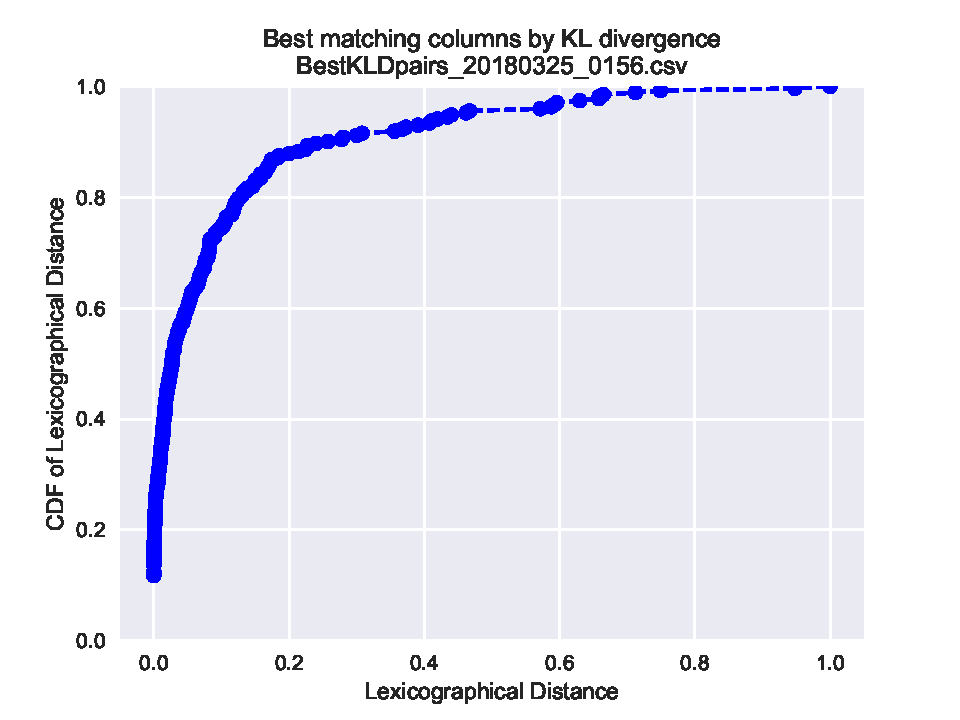
\includegraphics[trim={0 3mm 0 0},clip,width=1\columnwidth]{graphics/CDF_LexDistance1}
	\caption{CDF of Lexicographical Distance for the best match for each column.}
	\label{fig:cdflexdist}
	\trimfigurespacing
\end{figure}

We used Kullback-Leibler (KL) divergence to measure how one distribution diverges from from another. A KL divergence of 0 suggess that distributions could be similar, if not the same. A KL divergence of 1 suggests that two distributions are very different. If knowledge of a specific problem domain suggests that similarity of data distributions could be better represented by another measure, KL divergence can be easily swapped with for it in our system.  

Lexicographical Distance indicates the difference in the column labels of two distributions. We used two measures of Lexicographical Distance - Levenstein Distance and NGram Distance. Section~\ref{sec:expertui} talks about performance of both of the measures in estimating Lexicographical Distance on our dataset. A Lexicographical Distance value of 0 suggest that the two columns labels are exactly the same, whereas, a value of 1 suggests that the column labels are very different.

Learned heuristics require an assumption to build baseline match-quality functions. We proceed with the initial assumption that column pairs with \textit{similar} data would be labelled \textit{similarly}. The value of KL divergence of two columns is inversely proportional to \textit{similarity} of their data distributions. The value of Lexicographical distance of two columns is inversely proportional to \textit{similarity} of their column labels. We have verified this assumption by plotting the Cummulative Distribution Function of Lexicographical Distance of column pairs with minimum KL Divergence in Figure~\ref{fig:cdflexdist}. 80\% of column pairs with most similar data have their labels which are at most 0.129 lexical distance apart. This indicates that even without human intervention, columns pairs with the most similar data are already labelled similarly. 
 
For each distribution, we find the parameters ($\ell,h,\mu,\sigma,a$) that minimize the root-mean-squared (RMS) error between the theoritical and empirical distributions. 

$$\mathbb U(\ell, h)\;\;\;\;\;\mathbb N(\mu, \sigma)\;\;\;\;\;\mathbb Lognorm(\mu{*},\sigma{*})$$

Parameter estimation is performed by maximizing a log-likelihood function. Log-likelihood estimation is a widely used and robust technique for estimating the likelihood of a statistical distribution and its parameters being representative of the empirical data distribution. We implemented this using the SciPy package in Python. 

We then select the one distribution with the lowest overall RMS error. The resulting match-quality function is the probability of the column values being a representative sample drawn from this distribution.
% We measure this probability by the \placeholder{RMS Error} between the distribution of the sampled values and the distribution modeling the name.

\section{Expert Refinement}
\label{sec:expertui}
% -*- root: ../paper.tex -*-

While example data sets provide a good starting point for the \systemname knowledge-base, we anticipate that --- at least initially --- the training data will be too sparse to provide high quality matching suggestions.
To mitigate the effects of sparsity, \systemname relies on domain experts to curate its knowledge-base, refining existing matchers and defining new matching heuristics.
This is intended to be an ongoing process, with incremental feedback from experts and users continuously refining the knowledge-base.
In this section we outline the design of an interface that streamlines knowledge-base refinement, starting from a knowledge-base trained on example data.
The central elements of this interface are 
(1) Visualizing the current quality of the knowledge base;
(2) Identifying problem name/match-quality function pairs;
(3) Refining records in the knowledge base by removing or merging existing data, or adding expert knowledge.

\begin{figure}
	\centering
	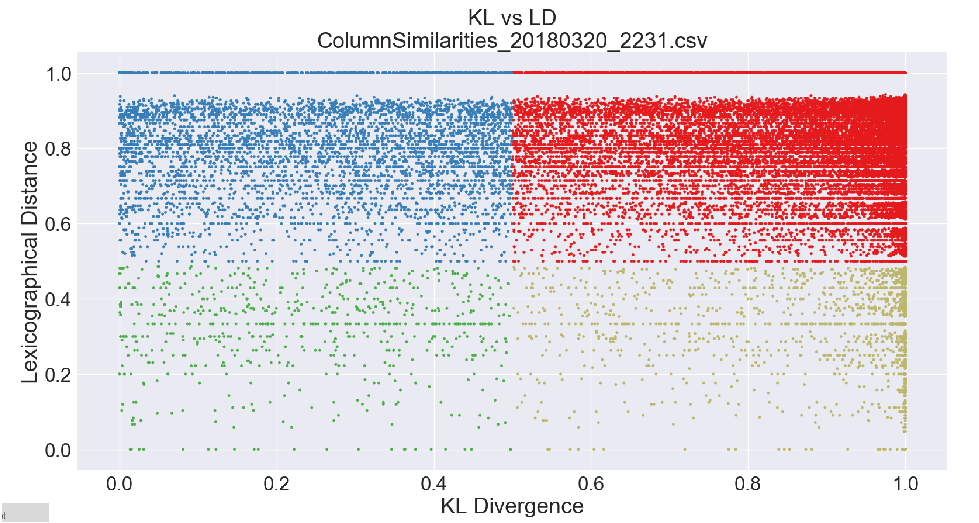
\includegraphics[width=1\columnwidth]{graphics/KBUI}
	\caption{Knowledge-base Editor: Showing Match Conflicts}
	\label{fig:editor:scatterplot}
\end{figure}

\subsection{Refinement Interface}
The initial goal of the \systemname editor is to help domain experts to quickly identify and resolve errors and redundancies in a preliminary knowlege-base freshly trained on new example data.  
The entry point into the refinement process is the \systemname editor's match-conflict explorer


\tinysection{Match Conflict Explorer}
This view, illustrated in Figure~\ref{fig:editor:scatterplot}., is a scatter plot, with each point corresponding to one pair of concepts.
The point's x- and y-coordinates express, respectively, how different the concepts and their related matchers are.
In both cases, a value of 0 indicates that the concepts (resp., the corresponding matchers) are identical, while a value of 1 indicates that the concepts (matchers) are completely different.
We refer to these as concept- and match-differences.
In this preliminary version of the system, we define concept-difference to be the lowest Levenshtein distance between any two names associated with each of the concepts.
We define the match difference as the lowest difference between any two matchers associated with each of the concepts, with inter-matcher differences defined based on their types.
For pairs of numerical distributions, this value is presently defined as the K/L-Divergence between the distributions.

The match conflict explorer helps to identify overlapping or erroneous matchers, as well as duplicate or overlapping concepts.
Specifically, the view is divided into four quadrants.  The lower-left, shown in green indicates high concept-similarity and highly overlapping matchers (true positives).  
The upper-right, shown in red indicates the reveerse (true negatives).
The upper-left, shown in blue identifies distinct concepts with similar matchers (potential false positives).  
The lower-right, shown in yellow identifies potentially similar concepts that have different matchers (potential false negatives).

\tinysection{Concept Pair View}
When a regions is selected in the explorer with a simple marquee tool, all pairs of concepts in the region are displayed to the user, along with their corresponding matchers.
\todo{mockup of the pair view}
A simple click on the scatter plot displays concept to the user, along with their corresponding matchers. User can analyze points in a dense area by using the zoom tool and then clicking on the point to get details.


\begin{figure}[H]
	\centering
	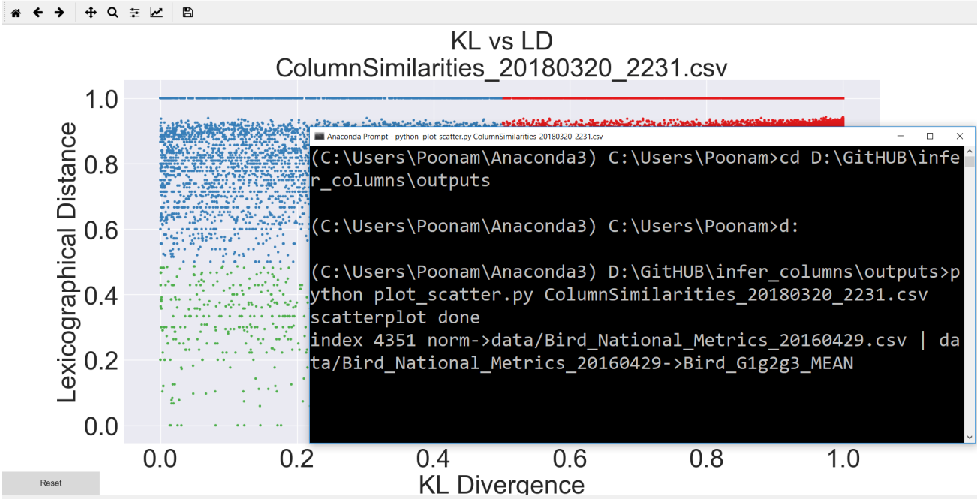
\includegraphics[width=0.8\columnwidth]{graphics/Pair_view}
	\caption{Pair view in scatter plot}
	\label{fig:Pair view}
\end{figure}


% \begin{figure}
% \begin{tabular}{r|l}
% \textbf{How Y modifies X} & $(\namesymbol_x \oplus \namesymbol_y)(T_A)$ \\\hline
% X Or Y & $max(\namesymbol_x(T_A), \namesymbol_y(T_A))$\\
% X And Y & $\namesymbol_x(T_A) \cdot \namesymbol_y(T_A)$\\
% X Unless Y & $min(\namesymbol_x(T_A), \namesymbol_y(T_A))$\\
% Y Instead of X & $\namesymbol_y(T_A)$\\
% Y Suggests X & $1-(1-\namesymbol_x(T_A))(1-\namesymbol_y(T_A))$
% \end{tabular}
% \caption{Example augmentation modifiers}
% \label{fig:modifiers}
% \end{figure}

% \tinysection{Modifiers}
% Expert knowledge in the knowledge-base is encoded in two parts: 
% (1) A quality-match function that provides a heuristic encoding of the expert knowledge, and 
% (2) An augmentation modifier that indicates how the new quality match function is to be combined with the existing one.  
% Figure~\ref{fig:modifiers} illustrates several example modifiers together with intuitive phrasings of each.  
% For example, if the expert heuristic defines an unrelated approach to matching columns, the highest match value is used.


\subsection{Understanding Refinement in Practice}
As experts identify errors or redundancies in the knowledge-base, they will need to patch the knowledge-base accordingly.
To better understand their needs in this process, we selected 200 \todo{that's an awfully specific number... why that?} concept pairs at random from among the potential false-positives and potential false-negatives.
We inspected each pair of concepts selected in this way and determined a root cause for each.
These root causes could each be described by one of six categories, summarized in Figure~\ref{fig:datatags:lowerright}.
We now discuss these categories in detail.

\begin{figure}
	\centering
	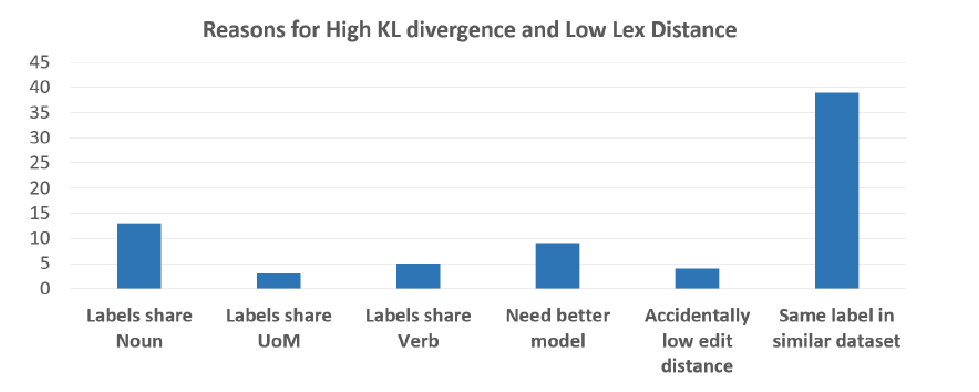
\includegraphics[width=0.8\columnwidth]{graphics/Lower_right_quad}
	\caption{Data tagging for points in lower right quadrant}
	\label{fig:datatags:lowerright}
\end{figure}
\todo{Font size on the figure!!}

\todo{Poonam: add graph for upper left quadrant}

\subsubsection{Need better model for training on examples}
For 9 pairs in the lower right quadrant and \todo{Poonam:add number} pairs in the upper left quadrant, the best fit matchers did not adequately describe the data distribution.
The training phase categorizes data by either uniform or normal distributions. 
However, we encountered distributions which can be described better using other distributions like zipfian or lognormal rather than normal or uniform.
\todo{The following sentence doesn't seem to be saying anything.  What was the outcome of the analysis?  Why is this a good example?  What's the takeaway?}
We analyzed the CDF(figure~\ref{fig:Distribution 1} and figure~\ref{fig:Distribution 2}) of data distribution for each column from the points identified from quadrant one and four of the scatter plot. 

\textbf{Resolution}: Although a more robust learning process might address this issue (e.g., by supporting more standard distributions like lognormal or zipfian), the only way to truly address this issue definitively is to allow experts to manually define custom distributions (e.g., using splines).

\begin{figure}[H]
	\centering
	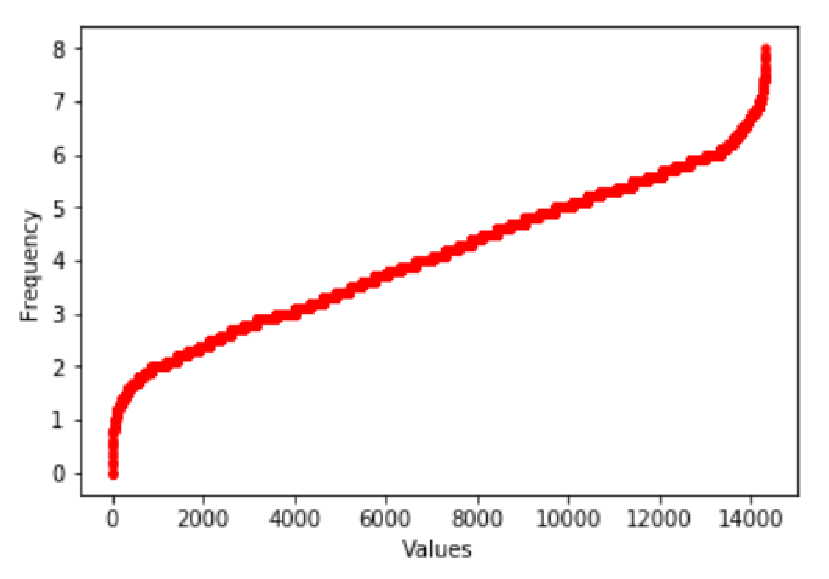
\includegraphics[width=0.8\columnwidth]{graphics/Challenge1_1}
	\caption{CDF of data distribution of column BIGGA\_AVG}
	\label{fig:Distribution 1}
\end{figure}

\begin{figure}[H]
	\centering
	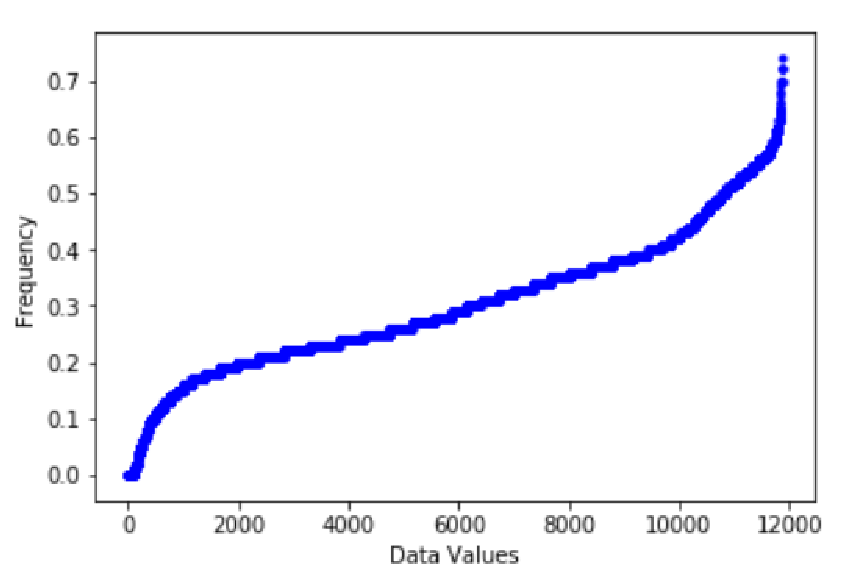
\includegraphics[width=0.8\columnwidth]{graphics/Challenge1_2}
	\caption{CDF of data distribution of column BIGGA\_AVG\_I}
	\label{fig:Distribution 2}
\end{figure}

\subsubsection{Same column name in a different context}
33 points, nearly half of the points sampled from among the potential false negatives, used the same name, but in different context.
For example, among the datasets used for this case study, we had two similar datasets in biodiversity domain. 
Both datasets consisted of data about flora and fauna, but from two different regions.

\textbf{Resolution}: Given the nature of the context, a domain expert may wish to unify both concepts or keep them separate.
In the former case, the expert needs to be able to merge concept nodes in the knowledge-base together.  
In the latter case, the expert needs to be able to override the concept-difference to mark them as being true negatives.

\subsubsection{Column names share measuring units}
Column names from the agriculture dataset shared measuring units like hectare and tonnes, these points (3 out of 79) resulted in different data distribution (high KL divergence) and low lexicographical distance due to measuring unit being present in the column names. For example: FRUITHECTARES and VEGHECTARES share the measuring units in the column names which causes the lexicographical distance to be low.

\textbf{Resolution}: Remove the measuring units from column names.

\subsubsection{Column names share noun}
Some of the column names (13 out of 79) had nouns in common. For instance, BigGameHunting\_RecreationDemand dataset has a column BG\_Demand and MigratoryBirdHunting\_RecreationDemand has a column MB\_Demand. Since the column names share noun, comparing these strings results in low lexicographical distance, but the data distribution are different.

\textbf{Resolution}: Remove the shared nouns from column names.


\subsubsection{Column names share verb}

Few column names had words like avg, mean, total, etc. appended at with the names. BAT\_AVG and TAVG share the verb AVG which results in in low lexicographical distance.

\textbf{Resolution}: Create a list of stop words and remove those from column names.

\subsubsection{Ngram Overestimation of column names}
Column WTFL\_AVG from biodiversity\_SW\_NHDPv2 and WET\_AG from Wet550\_2017 are classified as similar based on NGram comparison. 

\textbf{Resolution}: Use different string comparison function and compare the results.

\subsubsection{Columns with similar distributions but different names}
Out of 120 points analyzed from the upper left quadrant, \todo{Poonam:add number} had similar distributions as seen in~\ref{fig:Distribution 3} and~\ref{fig:Distribution 4} although the column names were different.

\textbf{Resolution}: The distributions were described as either uniform or normal, we can use other distributions (zipfian, lognorm) and compare the results. If the results are similar, then these columns can be deleted from the knowledge base.

\begin{figure}[H]
	\centering
	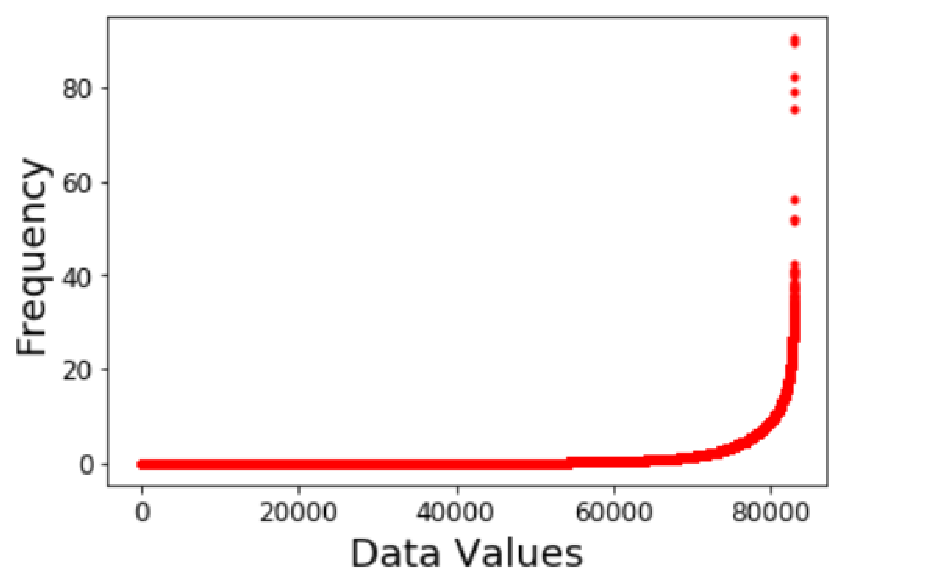
\includegraphics[width=0.8\columnwidth]{graphics/Challenge7_1}
	\caption{CDF of data distribution of column PctPasture\_slope9}
	\label{fig:Distribution 3}
\end{figure}

\begin{figure}[H]
	\centering
	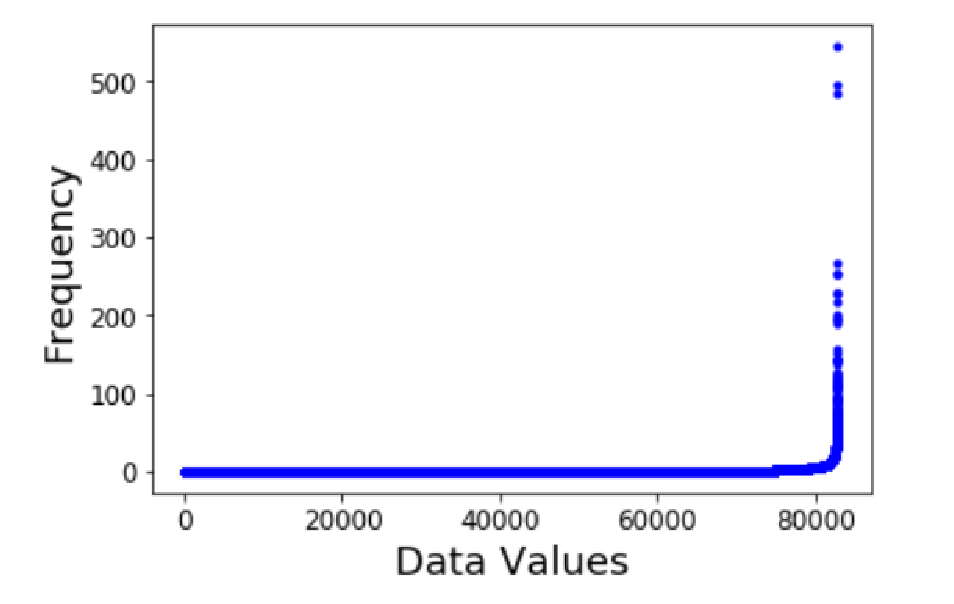
\includegraphics[width=0.8\columnwidth]{graphics/Challenge7_2}
	\caption{CDF of data distribution of column HistoricBuildings}
	\label{fig:Distribution 4}
\end{figure}


\subsection{Editor Interface}
Discuss what we've learned from the above and outline what capabilities the knowledge-base editing interface needs to expose:
\begin{enumerate*}
	\item Manual definition of data distributions
	\item Merge Concept Nodes
	\item Override concept difference: Force concepts to be distinct
	\item Override concept difference: Define stop-words
\end{enumerate*}


\section{Related Work}
\label{sec:related}
% -*- root: ../paper.tex -*-

Data distributions have been used for similar purposes in other work.  
For example GestureQuery~\cite{nandi2013gestural} uses data similarity between two attributes to select candidate attributes for an equi-join.  
To maximize the join arity, the system counts the number of times each value from one attribute appears in the other and a histogram is constructed from the counts for all of the values.

Wrangler \cite{kandel2011wrangler} and Potter's wheel \cite{raman2001potter} detect data domains through inclusion functions (e.g. regular expressions).
Wrangler in particular infers the data type of a column and highlights errors based on inconsistent data types. 
Wrangler also has several operators like split and unfold that create new columns.
The split operator decomposes composite data values into component distributions.  
The unfold operator reverses a table pivot, collapsing data laid out as key-value pairs into columns.  
A useful application of the \systemname knowledge-base that we hope to explore in future work is using it to detect opportunities for applying such operators.

% Although wrangler creates a new column for extracted data as part of unfold operation, but does not infer the column name, analyst has to name the new column manually.
% Unfold operation ”unflattens” tables; it takes two columns, collects rows that have the same values for all the other columns, and unfolds the two chosen columns. Values in one column are used as column names to align the values in the other column.

An orthogonal approach to modeling and matching columns is to use ontologies, which express entities, facts, relations between facts and properties of relations
Ontologies like Yago \cite{fabian2007yago} could be used to identify semantic properties that relate columns.

A data summary called the data describer is used in \cite{ping2017datasynthesizer}. The data types, correlations and distributions of the attributes in a private dataset are listed. Each attribute is categorized into either numerical or non-numerical. If non-numerical attribute cannot be parsed as datetime then it is considered to be a string.
\todo{What exactly is the purpose of the data describer.  How is it used?  How do its goals differ from ours, and what are the implications on its design?} 

PADS \cite{fisher2005pads} helps users to understand the layout and meaning of data by designing syntactic descriptions of the data.
Based on the syntax, accumulators track the number of good values, the number of bad values, and the distribution of legal values.
This technique could be used in \systemname to help capture expert knowledge.

There is an increasing number of datasets in which well-structured attributes
(with or without a name) can be identified, each containing a set of values called a domain. There is lack of schema description in most of the datasets.
LSH Ensemble is used in \cite{zhu2016lsh} to find domains that maximally contain a query dataset, which can help to find datasets that best augment a given set of data. 

\section{Future Work}
\label{sec:future}
Future work...

\bibliographystyle{ACM-Reference-Format}
\bibliography{main,oliver}

\end{document}
